\section{Examples}
\subsection{The tangent bundle of the 2-sphere}

We will define some higher inductive types to serve as domain and codomain of these motivating examples.

First we need a square, which will be a stand-in for a circle that can support a notion of a quarter-rotation. 

\begin{mydef}
The higher inductive type \( C_4 \) (where C stands for ``circle'').
\begin{align*}
C_4 &: \Type \\
c_1, c_2, c_3, c_4 &: C_4 \\
c_1c_2 &: c_1 = c_2 \\
c_2c_3 &: c_2 = c_3 \\
c_3c_4 &: c_3 = c_4 \\
c_4c_1 &: c_4 = c_1 \\
\end{align*}
\end{mydef}

\begin{tikzpicture}[
node distance = 15mm and 15mm,
V/.style = {circle, fill, draw=black, inner sep=1pt, font=\footnotesize},
every edge quotes/.style = {auto, font=\footnotesize},
arrow/.style={->,semithick}
]
\begin{scope}[nodes=V]
  \node[label=above left:\( c_1 \)] (1) {};
  \node[label=above right:\( c_2 \)] (2) [right=of 1]  {};
  \node[label=below right:\( c_3 \)] (3) [below=of 2]  {};
  \node[label=below left:\( c_4 \)] (4) [below=of 1]  {};
\end{scope}
\draw[arrow]
        (1)  edge["\( c_1c_2 \)"] (2)
        (2)  edge["\( c_2c_3 \)"] (3)
        (3)  edge["\( c_3c_4 \)"] (4)
        (4)  edge["\( c_4c_1 \)"] (1);
\end{tikzpicture}


We may also think of \( C_4 \) as the join of the two-element sets \( \{c_1, c_3\}* \{c_2, c_4\} \).

\begin{mydef}
The HIT \( \oo_0 \) is just 6 points, intended as the 0-skeleton of an octahedron, with vertices named after the colors on the faces of a Rubik's Cube.
\[ w, y, b, r, g, o : \oo_0 \]
\end{mydef}

\begin{mydef}
The HIT \( \oo_1 \) is the 1-skeleton of an octahedron.
\begin{align*}
w, y, b, r, g, o &: \oo_1 \\
wb &: w=b \\
wr &: w=r \\
wg &: w=g \\
wo &: w=o \\
yb &: y=b \\
yr &: y=r \\
yg &: y=g \\
yo &: y=o \\
br &: b=r \\
rg &: r=g \\
go &: g=o \\
ob &: o=b 
\end{align*}
\end{mydef}

\begin{mydef}
The HIT \( \oo \) which has 8 faces:
\begin{align*}
w, y, b, r, g, o &: \oo \\
wb &: w=b \\
wr &: w=r \\
wg &: w=g \\
wo &: w=o \\
yb &: y=b \\
yr &: y=r \\
yg &: y=g \\
yo &: y=o \\
br &: b=r \\
rg &: r=g \\
go &: g=o \\
ob &: o=b \\
wbr &: wb\cdot br\cdot wr^{-1} = \refl_w \\
wrg &: wr\cdot rg\cdot wg^{-1} = \refl_w \\
wgo &: wg\cdot go\cdot wo^{-1} = \refl_w \\
wob &: wo\cdot ob\cdot wb^{-1} = \refl_w \\
yrb &: yr\cdot rb\cdot yb^{-1} = \refl_y \\
ygr &: yg\cdot gr\cdot yr^{-1} = \refl_y \\
yog &: yo\cdot og\cdot yg^{-1} = \refl_y \\
ybo &: yb\cdot bo\cdot yo^{-1} = \refl_y
\end{align*}
\end{mydef}

\input{discrete_gauge_theory_oo_tikz}

We have obvious maps \( \oo_0\xrightarrow[]{i_0} \oo_1\xrightarrow[]{i_1} \oo \) that include each skeleton into the next-higher-dimensional skeleton.

Combinatorial spaces have a concept called the \emph{link} of a vertex, which will be the main tool by which we connect with manifold theory. The vertices in the link are the vertices that are one edge away from the given point, and the edges in the link are the edges connecting these. If the link of an \( n \)-dimensional combinatorial space is always a combinatorial \( n-1 \)-sphere, then we say the space is a \emph{combinatorial triangulation}. We will look only at HITs that have a link that is merely equivalent to \( C_4 \).

\begin{mydef}
If we have \( X:\Type \) then we define \( \BAut X\defeq \sit{Y:\Type} ||X=Y||_{-1} \). 
\end{mydef}

Denote by \( abcd:\BAut C_4 \) the HIT with vertices \( a, b, c, d \) and edges \( ab, bc, cd, da \) which clearly has various isomorphisms with \( C_4 \).

We can now define \( \link \) on the 0-skeleton. Extending this later on to the 1-skeleton and 2-skeleton will take us into differential geometry!

\begin{mydef}
\( \link:\oo_0\to\BAut C_4 \) is given by induction:
\begin{align*}
\link(w) &= brgo \\
\link(y) &= bogr \\
\link(b) &= woyr \\
\link(r) &= wbyg \\
\link(g) &= wryo \\
\link(o) &= wgyb
\end{align*}
We chose these orderings for the vertices by standing at the given vertex and enumerating the link in clockwise order, starting from \( w \) if possible, else \( b \).
\end{mydef}

Besides the link we also want to consider the 5-pointed object that includes the vertex itself and the edges connecting it to the vertices in the link. We will call such a shape an \emph{xbox} since it is a square with both diagonals. We will denote xboxes by extending the square notation with a fifth letter to indicate the center of the xbox. For example, we can define an xbox \( C_4c \) as follows:

\begin{mydef}
The higher inductive type \( C_4c \) with center \( c \), also denoted \( c_1c_2c_3c_4c \).
\begin{align*}
C_4c &: \Type \\
c_1, c_2, c_3, c_4, c &: C_4c \\
c_1c_2 &: c_1 = c_2 \\
c_2c_3 &: c_2 = c_3 \\
c_3c_4 &: c_3 = c_4 \\
c_4c_1 &: c_4 = c_1 \\
c_1c &: c_1 = c \\
c_2c &: c_2 = c \\
c_3c &: c_3 = c \\
c_4c &: c_4 = c 
\end{align*}
\end{mydef}

We can map our octahedron into the space of xboxes:
\begin{mydef}
\( \xbox:\oo_0\to\BAut C_4c \) is given by induction:
\begin{align*}
\xbox(w) &= brgow \\
\xbox(y) &= bogry \\
\xbox(b) &= woyrb \\
\xbox(r) &= wbygr \\
\xbox(g) &= wryog \\
\xbox(o) &= wgybo
\end{align*}
\end{mydef}

Finally we want to consider the 2-type that fills in the faces of the xbox. This is a contractible type we will call a \emph{disk}.

\begin{mydef}
The higher inductive type \( C_{4\disk} \) with center \( c \), also denoted \( c_1c_2c_3c_4c_\disk \).
\begin{align*}
C_{4\disk} &: \Type \\
c_1, c_2, c_3, c_4, c &: C_{4\disk} \\
c_1c_2 &: c_1 = c_2 \\
c_2c_3 &: c_2 = c_3 \\
c_3c_4 &: c_3 = c_4 \\
c_4c_1 &: c_4 = c_1 \\
c_1c &: c_1 = c \\
c_2c &: c_2 = c \\
c_3c &: c_3 = c \\
c_4c &: c_4 = c \\
c_1c_2c &: c_1c_2\cdot c_2c\cdot c_1c^{-1} = \refl \\
c_2c_3c &: c_2c_2\cdot c_3c\cdot c_2c^{-1} = \refl \\
c_3c_4c &: c_3c_2\cdot c_4c\cdot c_3c^{-1} = \refl \\
c_4c_1c &: c_4c_2\cdot c_1c\cdot c_4c^{-1} = \refl
\end{align*}
\end{mydef}

And we can map the octahedron into the space of disks:

\begin{mydef}
\( \disk:\oo_0\to\BAut C_{4\disk} \) is given by induction:
\begin{align*}
\xbox(w) &= brgow_\disk \\
\xbox(y) &= bogry_\disk \\
\xbox(b) &= woyrb_\disk \\
\xbox(r) &= wbygr_\disk \\
\xbox(g) &= wryog_\disk \\
\xbox(o) &= wgybo_\disk
\end{align*}
\end{mydef}

The idea of such combinatorial manifolds is that each point has a designated local disk and local sphere (and xbox) in the same way that a smooth manifold has an atlas. We want to proceed now to define bundles on this manifold. In HoTT that means constructing a map to a classifying space. The \( \link \) map will be our map, but we have only defined it on \( \oo_0 \).

Extending \( \link \) to the 1-skeleton requires new choices. We will choose a map inspired by the tangent bundle of the sphere, using the transport we can intuitively see through the embedding of \( \oo \) in 3-dimensional space as in our pictures. If you focus for a moment just on a path \( w\to b\to r \) and imagine rigidly tipping a moving equator along with a moving point, you can imagine a moving-equator point that starts at \( r \) and stays fixed when the north pole slides from \( w \) to \( b \). When the north pole continues sliding from \( b \) to \( r \) the moving-equator point moves to \( g \). Then it remains fixed when the north pole slides from \( r \) up to \( w \). So all in all we ``moved \( r \) to \( g \).'' When we track all the points on the original \( w \)-equator we see that we performed the rotation we earlier named \( R \).

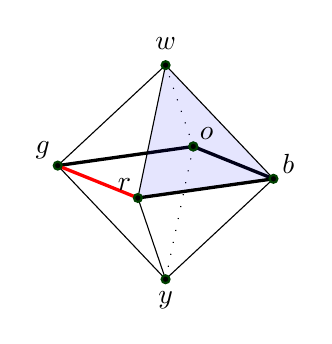
\begin{tikzpicture}%
  [x={(-0.860769cm, -0.121512cm)},
  y={(0.508996cm, -0.205391cm)},
  z={(-0.000053cm, 0.971107cm)},
  scale=1,
  eqback/.style={very thick},
  back/.style={loosely dotted, thin},
  eqedge/.style={very thick},
  edge/.style={black, thin},
  r/.style={red},
  facet/.style={fill=blue!95!black,fill opacity=0.1},
  vertex/.style={inner sep=1pt,circle,draw=green!25!black,fill=black,thick}]
\coordinate (-1, -1, 0) at (-1, -1, 0);
\coordinate (-1, 1, 0) at (-1, 1, 0);
\coordinate (0, 0, -1) at (0, 0, -1);
\coordinate (0, 0, 1) at (0, 0, 1);
\coordinate (1, -1, 0) at (1, -1, 0);
\coordinate (1, 1, 0) at (1, 1, 0);
%% Drawing edges in the back
%%
\draw[edge,eqback] (-1, -1, 0) -- (-1, 1, 0);
\draw[edge,back] (-1, -1, 0) -- (0, 0, -1.4);
\draw[edge,back] (-1, -1, 0) -- (0, 0, 1.4);
\draw[edge,eqback] (1, -1, 0) -- (-1, -1, 0);
%% Drawing vertices in the back
%%
\node[vertex] at (-1, -1, 0)     {};
%% Drawing the facets
%%
%\fill[facet] (1, 1, 0) -- (0, 0, -1.4) -- (1, -1, 0) -- cycle {};
%\fill[facet] (1, 1, 0) -- (0, 0, 1.4) -- (1, -1, 0) -- cycle {};
\fill[facet] (1, 1, 0) -- (-1, 1, 0) -- (0, 0, 1.4) -- cycle {};
%\fill[facet] (1, 1, 0) -- (-1, 1, 0) -- (0, 0, -1.4) -- cycle {};
%% Drawing edges in the front
%%
\draw[edge] (-1, 1, 0) -- (0, 0, -1.4);
\draw[edge] (-1, 1, 0) -- (0, 0, 1.4);
\draw[eqedge] (-1, 1, 0) -- (1, 1, 0);
\draw[edge] (0, 0, -1.4) -- (1, -1, 0);
\draw[edge] (0, 0, -1.4) -- (1, 1, 0);
\draw[edge] (0, 0, 1.4) -- (1, -1, 0);
\draw[edge] (0, 0, 1.4) -- (1, 1, 0);
\draw[r,eqedge] (1, 1, 0) -- (1, -1, 0);
%% Drawing the vertices in the front
%%
\begin{scope}[nodes=vertex]
\node[label=above right:\( b \)] at (-1, 1, 0)     {};
\node[label=below:\( y \)] at (0, 0, -1.4)     {};
\node[label=above:\( w \)] at (0, 0, 1.4)     {};
\node[label=above left:\( g \)] at (1, -1, 0)     {};
\node[label=above left:\( r \)] at (1, 1, 0)     {};
\node[label=above right:\( o \)] at (-1, -1, 0)     {};
\end{scope}
\end{tikzpicture}
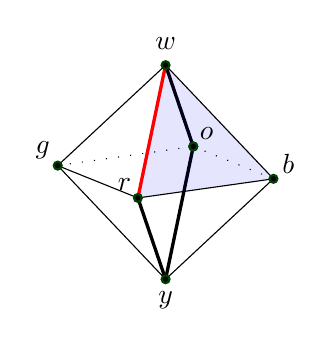
\begin{tikzpicture}%
  [x={(-0.860769cm, -0.121512cm)},
  y={(0.508996cm, -0.205391cm)},
  z={(-0.000053cm, 0.971107cm)},
  scale=1,
  eqback/.style={very thick},
  back/.style={loosely dotted, thin},
  eqedge/.style={very thick},
  r/.style={red},
  edge/.style={black, thin},
  facet/.style={fill=blue!95!black,fill opacity=0.1},
  vertex/.style={inner sep=1pt,circle,draw=green!25!black,fill=black,thick}]
\coordinate (-1, -1, 0) at (-1, -1, 0);
\coordinate (-1, 1, 0) at (-1, 1, 0);
\coordinate (0, 0, -1) at (0, 0, -1);
\coordinate (0, 0, 1) at (0, 0, 1);
\coordinate (1, -1, 0) at (1, -1, 0);
\coordinate (1, 1, 0) at (1, 1, 0);
%% Drawing edges in the back
%%
\draw[edge,back] (-1, -1, 0) -- (-1, 1, 0);
\draw[edge,eqback] (-1, -1, 0) -- (0, 0, -1.4);
\draw[edge,eqback] (0, 0, 1.4) -- (-1, -1, 0);
\draw[edge,back] (1, -1, 0) -- (-1, -1, 0);
%% Drawing vertices in the back
%%
\node[vertex] at (-1, -1, 0)     {};
%% Drawing the facets
%%
% \fill[facet] (1, 1, 0) -- (0, 0, -1.4) -- (1, -1, 0) -- cycle {};
% \fill[facet] (1, 1, 0) -- (0, 0, 1.4) -- (1, -1, 0) -- cycle {};
\fill[facet] (1, 1, 0) -- (-1, 1, 0) -- (0, 0, 1.4) -- cycle {};
% \fill[facet] (1, 1, 0) -- (-1, 1, 0) -- (0, 0, -1.4) -- cycle {};
%% Drawing edges in the front
%%
\draw[edge] (-1, 1, 0) -- (0, 0, -1.4);
\draw[edge] (-1, 1, 0) -- (0, 0, 1.4);
\draw[edge] (-1, 1, 0) -- (1, 1, 0);
\draw[edge] (0, 0, -1.4) -- (1, -1, 0);
\draw[eqedge] (0, 0, -1.4) -- (1, 1, 0);
\draw[edge] (0, 0, 1.4) -- (1, -1, 0);
\draw[r,eqedge] (1, 1, 0) -- (0, 0, 1.4) ;
\draw[edge] (1, 1, 0) -- (1, -1, 0);
%% Drawing the vertices in the front
%%
\begin{scope}[nodes=vertex]
\node[label=above right:\( b \)] at (-1, 1, 0)     {};
\node[label=below:\( y \)] at (0, 0, -1.4)     {};
\node[label=above:\( w \)] at (0, 0, 1.4)     {};
\node[label=above left:\( g \)] at (1, -1, 0)     {};
\node[label=above left:\( r \)] at (1, 1, 0)     {};
\node[label=above right:\( o \)] at (-1, -1, 0)     {};
\end{scope}
\end{tikzpicture}
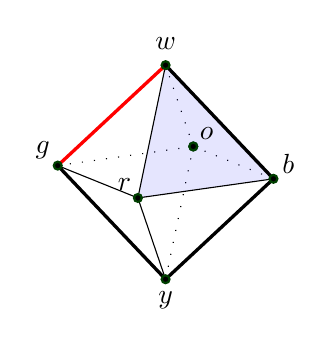
\begin{tikzpicture}%
  [x={(-0.860769cm, -0.121512cm)},
  y={(0.508996cm, -0.205391cm)},
  z={(-0.000053cm, 0.971107cm)},
  scale=1,
  eqback/.style={very thick},
  back/.style={loosely dotted, thin},
  eqedge/.style={very thick},
  r/.style={red},
  edge/.style={black, thin},
  facet/.style={fill=blue!95!black,fill opacity=0.1},
  vertex/.style={inner sep=1pt,circle,draw=green!25!black,fill=black,thick}]
\coordinate (-1, -1, 0) at (-1, -1, 0);
\coordinate (-1, 1, 0) at (-1, 1, 0);
\coordinate (0, 0, -1) at (0, 0, -1);
\coordinate (0, 0, 1) at (0, 0, 1);
\coordinate (1, -1, 0) at (1, -1, 0);
\coordinate (1, 1, 0) at (1, 1, 0);
%% Drawing edges in the back
%%
\draw[edge,back] (-1, -1, 0) -- (-1, 1, 0);
\draw[edge,back] (-1, -1, 0) -- (0, 0, -1.4);
\draw[edge,back] (-1, -1, 0) -- (0, 0, 1.4);
\draw[edge,back] (1, -1, 0) -- (-1, -1, 0);
%% Drawing vertices in the back
%%
\node[vertex] at (-1, -1, 0)     {};
%% Drawing the facets
%%
% \fill[facet] (1, 1, 0) -- (0, 0, -1.4) -- (1, -1, 0) -- cycle {};
% \fill[facet] (1, 1, 0) -- (0, 0, 1.4) -- (1, -1, 0) -- cycle {};
\fill[facet] (1, 1, 0) -- (-1, 1, 0) -- (0, 0, 1.4) -- cycle {};
% \fill[facet] (1, 1, 0) -- (-1, 1, 0) -- (0, 0, -1.4) -- cycle {};
%% Drawing edges in the front
%%
\draw[eqedge] (-1, 1, 0) -- (0, 0, -1.4);
\draw[eqedge] (0, 0, 1.4) -- (-1, 1, 0);
\draw[edge] (-1, 1, 0) -- (1, 1, 0);
\draw[eqedge] (0, 0, -1.4) -- (1, -1, 0);
\draw[edge] (0, 0, -1.4) -- (1, 1, 0);
\draw[r,eqedge] (1, -1, 0) -- (0, 0, 1.4);
\draw[edge] (0, 0, 1.4) -- (1, 1, 0);
\draw[edge] (1, 1, 0) -- (1, -1, 0);
%% Drawing the vertices in the front
%%
\begin{scope}[nodes=vertex]
\node[label=above right:\( b \)] at (-1, 1, 0)     {};
\node[label=below:\( y \)] at (0, 0, -1.4)     {};
\node[label=above:\( w \)] at (0, 0, 1.4)     {};
\node[label=above left:\( g \)] at (1, -1, 0)     {};
\node[label=above left:\( r \)] at (1, 1, 0)     {};
\node[label=above right:\( o \)] at (-1, -1, 0)     {};
\end{scope}
\end{tikzpicture}
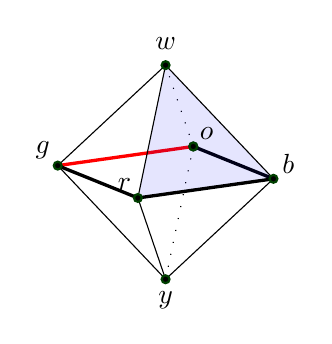
\begin{tikzpicture}%
  [x={(-0.860769cm, -0.121512cm)},
  y={(0.508996cm, -0.205391cm)},
  z={(-0.000053cm, 0.971107cm)},
  scale=1,
  eqback/.style={very thick},
  back/.style={loosely dotted, thin},
  eqedge/.style={very thick},
  edge/.style={black, thin},
  r/.style={red},
  facet/.style={fill=blue!95!black,fill opacity=0.1},
  vertex/.style={inner sep=1pt,circle,draw=green!25!black,fill=black,thick}]
\coordinate (-1, -1, 0) at (-1, -1, 0);
\coordinate (-1, 1, 0) at (-1, 1, 0);
\coordinate (0, 0, -1) at (0, 0, -1);
\coordinate (0, 0, 1) at (0, 0, 1);
\coordinate (1, -1, 0) at (1, -1, 0);
\coordinate (1, 1, 0) at (1, 1, 0);
%% Drawing edges in the back
%%
\draw[edge,eqback] (-1, -1, 0) -- (-1, 1, 0);
\draw[edge,back] (-1, -1, 0) -- (0, 0, -1.4);
\draw[edge,back] (-1, -1, 0) -- (0, 0, 1.4);
\draw[edge,eqback,r] (1, -1, 0) -- (-1, -1, 0);
%% Drawing vertices in the back
%%
\node[vertex] at (-1, -1, 0)     {};
%% Drawing the facets
%%
% \fill[facet] (1, 1, 0) -- (0, 0, -1.4) -- (1, -1, 0) -- cycle {};
% \fill[facet] (1, 1, 0) -- (0, 0, 1.4) -- (1, -1, 0) -- cycle {};
\fill[facet] (1, 1, 0) -- (-1, 1, 0) -- (0, 0, 1.4) -- cycle {};
% \fill[facet] (1, 1, 0) -- (-1, 1, 0) -- (0, 0, -1.4) -- cycle {};
%% Drawing edges in the front
%%
\draw[edge] (-1, 1, 0) -- (0, 0, -1.4);
\draw[edge] (-1, 1, 0) -- (0, 0, 1.4);
\draw[eqedge] (-1, 1, 0) -- (1, 1, 0);
\draw[edge] (0, 0, -1.4) -- (1, -1, 0);
\draw[edge] (0, 0, -1.4) -- (1, 1, 0);
\draw[edge] (0, 0, 1.4) -- (1, -1, 0);
\draw[edge] (0, 0, 1.4) -- (1, 1, 0);
\draw[eqedge] (1, 1, 0) -- (1, -1, 0);
%% Drawing the vertices in the front
%%
\begin{scope}[nodes=vertex]
\node[label=above right:\( b \)] at (-1, 1, 0)     {};
\node[label=below:\( y \)] at (0, 0, -1.4)     {};
\node[label=above:\( w \)] at (0, 0, 1.4)     {};
\node[label=above left:\( g \)] at (1, -1, 0)     {};
\node[label=above left:\( r \)] at (1, 1, 0)     {};
\node[label=above right:\( o \)] at (-1, -1, 0)     {};
\end{scope}
\end{tikzpicture}


In general we have:
\begin{mydef}
Define \( T_1:\oo\to\BAutoso \) on just the 1-skeleton by extending \( T_0 \) as follows:
Transport away from \( w \):
\begin{itemize}
\item \( T_1(wb):[b, r, g, o]\mapsto [y, r, w, o] \) (\( r, o \) fixed)
\item \( T_1(wr):[b, r, g, o]\mapsto [b, y, g, w] \) (\( b, g \) fixed)
\item \( T_1(wg):[b, r, g, o]\mapsto [w, r, y, o] \)
\item \( T_1(wo):[b, r, g, o]\mapsto [b, w, g, y] \)
\end{itemize}
Transport away from \( y \):
\begin{itemize}
\item \( T_1(yb):[b, o, g, r]\mapsto [w, o, y, r] \)
\item \( T_1(yr):[b, o, g, r]\mapsto [b, y, g, w] \)
\item \( T_1(yg):[b, o, g, r]\mapsto [y, o, w, r] \)
\item \( T_1(yo):[b, o, g, r]\mapsto [b, w, g, y] \)
\end{itemize}
Transport along the equator:
\begin{itemize}
\item \( T_1(br):[w, o, y, r]\mapsto [w, b, y, g] \) 
\item \( T_1(rg):[w, b, y, g]\mapsto [w, r, y, o] \)
\item \( T_1(go):[w, r, y, o]\mapsto [w, g, y, b] \)
\item \( T_1(ob):[w, g, y, b]\mapsto [w, o, y, r] \)
\end{itemize}
\end{mydef}

At this point we have defined a map on the 1-skeleton of \( \oo \).

\begin{myclaim}
\( T_1 \) defines a principal circle bundle with connection over the 1-skeleton of \( \oo \).
\end{myclaim}

We now want to extend this map to all of \( \oo \) by providing values for the eight faces. Here we will be guided by the classical relationship between a connection and its curvature. The curvature is computed from the connection, it doesn't contain any new data. Classically the integral of curvature over a 2-cell is the holonomy given by transport around the boundary. 

\begin{mydef}
Define \( T_2:\oo\to\BAutoso \) by extending \( T_1 \) as follows. We will send every clockwise triangle to \( R' \), the homotopy from \( \refl \) to \( R \):
\begin{itemize}
\item \( T_2(wbr)=R' \) 
\item \( T_2(wrg)=R' \)
\item \( T_2(wgo)=R' \)
\item \( T_2(ybo)=R' \)
\item \( T_2(yrb)=R' \) 
\item \( T_2(ygr)=R' \)
\item \( T_2(yog)=R' \)
\item \( T_2(ybo)=R' \)
\end{itemize}
\end{mydef}


\subsection{Combinatorial manifolds}

(This section is not quite off the ground.)

The combinatorial structure we have in mind is a nerve of a good open cover. What do we know about which smooth manifolds have such covers? While we're at it, let's survey all the combinatorial-flavored spaces and survey what smooth manifolds are homotopy equivalent to which structures.

What topological manifolds are equivalent to a CW complex? The answer is the composition of a few results summarized by Allen Hatcher\footnote{\url{https://mathoverflow.net/questions/201944/topological-n-manifolds-have-the-homotopy-type-of-n-dimensional-cw-complexes}} (citing \cite{kirby_siebenmann} and \cite{freedman_quinn}):

\begin{quote}
Every topological manifold has a handlebody structure except in dimension 4, where a 4-manifold has a handlebody structure if and only if it is smoothable. This is a theorem on page 136 of Freedman and Quinn's book ``Topology of 4-Manifolds'', with a reference given to the Kirby-Siebenmann book for the higher-dimensional case. It is then an elementary fact that an \( n \)-manifold with a handlebody structure is homotopy equivalent to a CW complex with one \( k \)-cell for each \( k \)-handle, so in particular there are no cells of dimension greater than \( n \). At least in the compact case a manifold with a handlebody structure is in fact homeomorphic to a CW complex with \( k \)-cells corresponding to \( k \)-handles; see page 107 of Kirby-Siebenmann. This probably holds in the noncompact case as well, though I don't know a reference.
\end{quote}


